%------------------------------------------------------------------------------%
\section{Metodología}
%------------------------------------------------------------------------------%

Se ha usado una metodología ágil híbrida para el desarrollo del proyecto de SCRUM, LEAN y KANBAN.  

Las metodologías ágiles permiten un desarrollo incremental. Sus principales
características es que se apoyan en los individuos e interacciones y le dan preferencia a versiones ejecutables desde el inicio del proyecto, que se van incrementando de forma iterativa \parencite{pmi2017}. 

SCRUM es una metodología orientada al desarrollo de software en equipos pequeños, idealmente de hasta 10 personas. Se caracteriza son los llamados \textit{sprints}, los cuales consisten en tareas asignadas a etapas de usualmente dos semanas y la estructura de los roles que se sigue en este proyecto \parencite{schwaber2020}.

KANBAN es un sistema de organización de tareas que se utiliza junto con SCRUM en el cual las tareas suelen escribirse en tarjetas agrupadas en categorías de acuerdo al estado de la tarea —en proceso, por planificar, terminado, etc— cuando se combina con SCRUM se suele escribir el sprint al cual pertenecen las tareas. Las tarjetas suelen ser virtuales \parencite{stellman2014}. 

LEAN es un marco de valores que promueve ``la organización de las actividades humanas para entregar más beneficios a la sociedad y al individuo, eliminando los despilfarros'' \parencite{womack2003}. En la \figura{fig:penasmientolean} se describe un poco estos valores.

\begin{figure}
    \centering
    \caption[Pensamiento LEAN]{Valores LEAN en el desarollo de software: \textit{1. Eliminar el despilfarro} evitar requerimientos procesos y funciones innecesarias, cambiar equipo, etc. \textit{2. Ampliar el aprendizaje} dedicar recursos a la mejora de las habilidades. \textit{3. Posponer decisiones} así se evitan discusiones largas y pérdidas de tiempo. \textit{4. Liberar pronto} versiones para poder tener retroalimentación de los usuarios y el cliente. \textit{5. Empoderar al equipo} promocionar la autonomía, asumir que todos saben hacer su trabajo. \textit{6. Construir calidad} debe ser el corazón del proyecto de inicio a fin. \textit{7. Optimizar el sistema} implementar métodos de medición para optimizar procesos en cada iteración.}
    \label{fig:penasmientolean}
    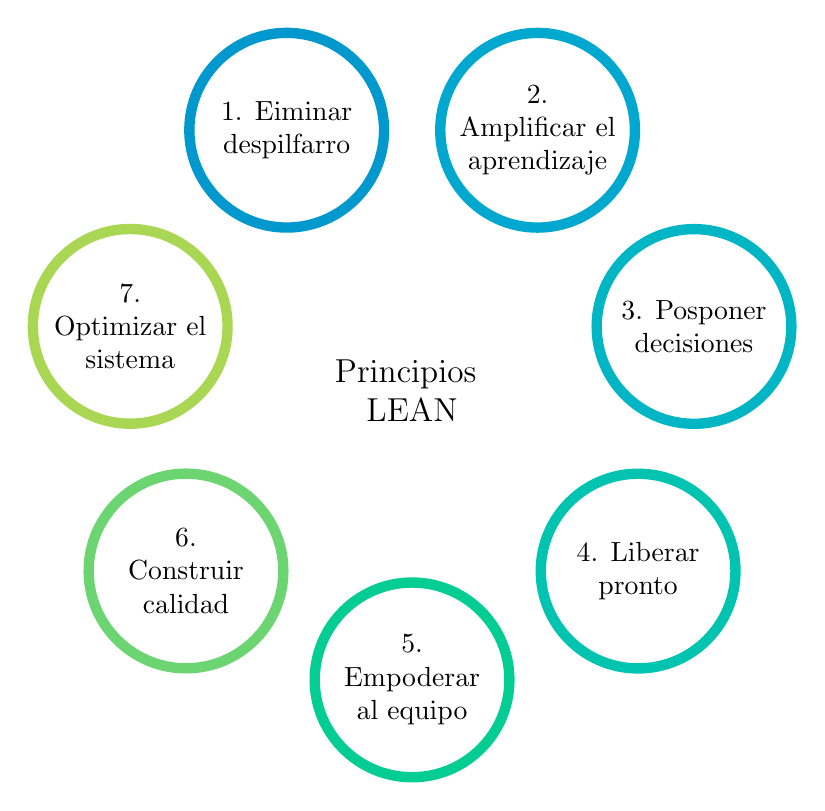
\begin{tikzpicture}[x=0.75pt,y=0.75pt,yscale=-1,xscale=1]
%uncomment if require: \path (0,399); %set diagram left start at 0, and has height of 399

%Flowchart: Connector [id:dp6671534120935239] 
\draw  [color={rgb, 255:red, 0; green, 152; blue, 205 }  ,draw opacity=1 ][line width=3.75]  (192.38,68.52) .. controls (192.38,42.62) and (213.38,21.62) .. (239.29,21.62) .. controls (265.19,21.62) and (286.19,42.62) .. (286.19,68.52) .. controls (286.19,94.42) and (265.19,115.42) .. (239.29,115.42) .. controls (213.38,115.42) and (192.38,94.42) .. (192.38,68.52) -- cycle ;
%Flowchart: Connector [id:dp9742464437933368] 
\draw  [color={rgb, 255:red, 0; green, 168; blue, 207 }  ,draw opacity=1 ][line width=3.75]  (313.27,68.54) .. controls (313.27,42.64) and (334.27,21.64) .. (360.17,21.64) .. controls (386.08,21.64) and (407.07,42.64) .. (407.07,68.54) .. controls (407.07,94.45) and (386.08,115.44) .. (360.17,115.44) .. controls (334.27,115.44) and (313.27,94.45) .. (313.27,68.54) -- cycle ;
%Flowchart: Connector [id:dp17986667998434147] 
\draw  [color={rgb, 255:red, 0; green, 182; blue, 197 }  ,draw opacity=1 ][line width=3.75]  (388.63,163.07) .. controls (388.63,137.17) and (409.63,116.17) .. (435.53,116.17) .. controls (461.43,116.17) and (482.43,137.17) .. (482.43,163.07) .. controls (482.43,188.97) and (461.43,209.97) .. (435.53,209.97) .. controls (409.63,209.97) and (388.63,188.97) .. (388.63,163.07) -- cycle ;
%Flowchart: Connector [id:dp49064716171042055] 
\draw  [color={rgb, 255:red, 0; green, 195; blue, 176 }  ,draw opacity=1 ][line width=3.75]  (361.7,280.92) .. controls (361.7,255.02) and (382.7,234.02) .. (408.6,234.02) .. controls (434.51,234.02) and (455.5,255.02) .. (455.5,280.92) .. controls (455.5,306.83) and (434.51,327.83) .. (408.6,327.83) .. controls (382.7,327.83) and (361.7,306.83) .. (361.7,280.92) -- cycle ;
%Flowchart: Connector [id:dp4374690028497701] 
\draw  [color={rgb, 255:red, 4; green, 205; blue, 147 }  ,draw opacity=1 ][line width=3.75]  (252.78,333.35) .. controls (252.78,307.45) and (273.77,286.45) .. (299.68,286.45) .. controls (325.58,286.45) and (346.58,307.45) .. (346.58,333.35) .. controls (346.58,359.26) and (325.58,380.25) .. (299.68,380.25) .. controls (273.77,380.25) and (252.78,359.26) .. (252.78,333.35) -- cycle ;
%Flowchart: Connector [id:dp9167083401815027] 
\draw  [color={rgb, 255:red, 109; green, 212; blue, 114 }  ,draw opacity=1 ][line width=3.75]  (143.87,280.88) .. controls (143.87,254.98) and (164.87,233.98) .. (190.77,233.98) .. controls (216.67,233.98) and (237.67,254.98) .. (237.67,280.88) .. controls (237.67,306.78) and (216.67,327.78) .. (190.77,327.78) .. controls (164.87,327.78) and (143.87,306.78) .. (143.87,280.88) -- cycle ;
%Flowchart: Connector [id:dp24671509877720965] 
\draw  [color={rgb, 255:red, 169; green, 215; blue, 83 }  ,draw opacity=1 ][line width=3.75]  (116.99,163.02) .. controls (116.99,137.12) and (137.99,116.12) .. (163.89,116.12) .. controls (189.8,116.12) and (210.79,137.12) .. (210.79,163.02) .. controls (210.79,188.92) and (189.8,209.92) .. (163.89,209.92) .. controls (137.99,209.92) and (116.99,188.92) .. (116.99,163.02) -- cycle ;

% Text Node
\draw (239.29,68.52) node   [align=left] {\begin{minipage}[lt]{54.92pt}\setlength\topsep{0pt}
\begin{center}
1. Eiminar\\despilfarro
\end{center}

\end{minipage}};
% Text Node
\draw (360.17,68.54) node   [align=left] {\begin{minipage}[lt]{58.29pt}\setlength\topsep{0pt}
\begin{center}
2. \\Amplificar el\\aprendizaje
\end{center}

\end{minipage}};
% Text Node
\draw (435.53,163.07) node   [align=left] {\begin{minipage}[lt]{57.75pt}\setlength\topsep{0pt}
\begin{center}
3. Posponer\\decisiones
\end{center}

\end{minipage}};
% Text Node
\draw (408.6,280.92) node   [align=left] {\begin{minipage}[lt]{48.68pt}\setlength\topsep{0pt}
\begin{center}
4. Liberar \\pronto
\end{center}

\end{minipage}};
% Text Node
\draw (299.68,333.35) node   [align=left] {\begin{minipage}[lt]{53.21pt}\setlength\topsep{0pt}
\begin{center}
5.\\Empoderar\\al equipo
\end{center}

\end{minipage}};
% Text Node
\draw (190.77,280.88) node   [align=left] {\begin{minipage}[lt]{46.95pt}\setlength\topsep{0pt}
\begin{center}
6.\\Construir \\calidad
\end{center}

\end{minipage}};
% Text Node
\draw (163.89,163.02) node   [align=left] {\begin{minipage}[lt]{57.15pt}\setlength\topsep{0pt}
\begin{center}
7.\\Optimizar el\\sistema
\end{center}

\end{minipage}};
% Text Node
\draw (299.7,194.04) node  [font=\large] [align=left] {\begin{minipage}[lt]{55.79pt}\setlength\topsep{0pt}
Principios
\begin{center}
LEAN
\end{center}

\end{minipage}};


\end{tikzpicture}

    \source{Elaboración propia con información de \figurecite{ferreit2021}.}
  \end{figure}
  

\subsection{Roles}

Los roles del proyecto están asignados de acuerdo a la metodología SCRUM. Debido a lo pequeño del equipo de trabajo los autores ocupan varios de los roles.

\begin{itemize}
  \item \textit{Product Owner} Responsable de maximizar el valor del producto final: \atsecondauthor.
  \item \textit{Scrum Master} Encargado de la planificación y el entendimiento de la metodología SCRUM: \atfirstauthor
  \item \textit{Development Team Mebers}: Ambos autores.
\end{itemize}


\subsection{\textit{Sprints}}
\label{sec:sprints}

Se definió que la duración de cada \textit{sprint} para este proyecto fuera de una semana. Un \textit{sprint} consta de las siguientes ceremonias:


\begin{itemize}
  \item Planificación: se define que se hará durante el \textit{sprint} — 1 hora al inicio del mismo.
  \item Implementación: el trabajo en si mismo —3 días de trabajo, y 1 día de pruebas, con un día liberación.  
  \item Demostración y revisión —se presenta el trabajo y se presentan comentarios y partes a corregir —reunión de 1 hora.
  \item Retrospectiva: se presenta una versión del trabajo con correcciones —reunión de 1 hora. 
  \item Refinamiento: revisión de historias existentes, adición de nuevas historias.
\end{itemize}


\subsection{\textit{Historias Iniciales}}

Las historias se definieron en Azure. Se pueden consultar a detalle en \href{https://dev.azure.com/petartificialvision}{petartificialvision}. Aquí presentamos una tabla con las historias.

\begin{landscape}
    \begin{small}
    \begin{longtable}{
        p{0.04\lanscapetablewidth}p{0.11\lanscapetablewidth}p{0.18\lanscapetablewidth}p{0.36\lanscapetablewidth}p{0.07\lanscapetablewidth}p{0.14\lanscapetablewidth}p{0.11\lanscapetablewidth}
    }
        \caption{Historias iniciales del proyecto.}\label{tab:historias}\\
        \toprule
        ID &
        Tipo de historia &
        Título &
        Descripción &
        Puntos de esfuerzo &
        Asignado a &
        Estado \\
        \midrule
        \endfirsthead
        \caption*{\textbf{\textup{Tabla \ref*{tab:historias} Continuación.}}  Historias iniciales del proyecto.}\\
        \toprule
        ID &
        Tipo de historia &
        Título &
        Descripción &
        Puntos de esfuerzo &
        Asignado a &
        Estado \\
        \midrule        
        \endhead
        \midrule\multicolumn{7}{r}{\itshape Continua en la siguiente página.}\\\endfoot
        \bottomrule\endlastfoot
        2 &
        Tarea &
        Entrevistar usuarios &
        Como product owner quiero aplicar la entrevista creada en la tarea Tarea 10: Diseñar entrevista para obtener retroalimentación para usuarios. - Boards (azure.com) a al menos 15 posibles usuarios de la aplicación. &
        7 &
        \atfirstauthor &
        Terminado \\
        4 &
        Tarea &
        Desarrollar código para acceder a la camara. &
        Como desarrollador quiero crear un segmento de código que me permita acceder a una camára web (si el dispositivo la tiene) desde un programa de python, una vez que se acceda a la camára quiero poder pasar el vídeo desde la camára a otros segmentos de código. &
        11 &
        \atfirstauthor &
        Por Hacer \\
        6 &
        Tarea &
        Entrenar red neuronal para segmentación de imágenes. &
        Como desarrollador quiero entrenar la red neuronal seleccionada en  para segmentar automáticamente imágenes. &
        17 &
        \atsecondauthor &
        Por Hacer \\
        7 &
        Tarea &
        Desarrollar detector de movimiento &
        Como desarrollador quiero crear un segmento de código que permita detectar movimiento en un segmento de vídeo.  &
        13 &
        \atfirstauthor &
        Por Hacer \\
        10 &
        Tarea &
        Diseñar entrevista para obtener retroalimentación para usuarios. &
        Yo como product owner quiero diseñar una entrevista que me permita obtener retroalimentación de los usuarios, está entrevista debe estar publicada en google forms para que los usuarios puedan acceder fácilmente a ella. &
        5 &
        \atfirstauthor &
        Terminado \\
        11 &
        Tarea &
        Entrevistar Usuarios. &
        {} &
        {} &
        \atfirstauthor &
        Por Hacer \\
        12 &
        Tarea &
        Investigar opciones para la segmentación de imágenes. &
        Yo como desarrollador quiero investigar las posibles opciones existentes para realizar segmentación de imágenes automática. Debo recabar las posibles opciones y presentarlas en la reunión de refinamiento del siguiente sprint (una vez terminada esta historia). &
        5 &
        \atsecondauthor &
        Por Hacer \\
        18 &
        Tarea &
        Detección de suelos. &
        Como desarrollador quiero desarrollar una red neuronal y entrenarla para detectar suelos. &
        17 &
        \atsecondauthor &
        Terminado \\
    \end{longtable} 
\end{small}
\end{landscape}


\subsection{Gestión de historias}

Se ha ocupado Azure Devops debido a su integración con GiHub y su amplio abanico de herramientas gratuitas para la administración de equipos, así mismo tiene una excelente integración con todo el ecosistema Microsoft.

\subsection{Puntos de esfuerzo}

Los puntos de esfuerzo se han asignado a cada historia ocupando el modelo de números primos, donde el esfuerzo de una historia se mide usando números primos, lo que provoca que el crecimiento de esfuerzo no sea lineal y permite observar mejor si una historia debe ser dividida o simplificada al tener esfuerzos muy grandes.

\subsection{Etapas LEAN}

Las etapas del inicio de un proyecto siguiendo los principios LEAN son las siguientes \parencite{cardenas}.

\subsubsection{Propón una hipótesis}

Esta etapa esta relacionada con el objetivo del trabajo \hyperref[sec:objetivos]{objetivo del trabajo}, que se puede escribir en forma de hipótesis como:

\begin{quotebox}
Hay personas dispuestas a comprar un sistema inteligente de vigilancia de mascotas.
\end{quotebox}

\subsubsection{Valida la hipótesis}

Se realizó en parte en el \hyperref[sec:desarrolloconceptual]{desarollo conceptual}. La hipótesis se validó con un prototipo que fue mostrado al público. La hipótesis se seguirá verificando mostrando y obteniendo la retroalimentación de los usuarios.

\subsubsection{Mide la hipótesis}

Esta etapa se explica en la \seccion{sec:mediciones}.

\subsubsection{Aprende del proceso}

Dentro de LEAN, se pide mejorar el proceso con la retroalimentación de los clientes, incluso cambiar la hipótesis. Esto será vital durante el desarrollo del proyecto.

\subsection{Mediciones}
\label{sec:mediciones}

Las mediciones se harán al inicio de cada \textit{sprint}. Para medir la calidad se establecerá un esfuerzo objetivo que se contrastará con la evaluación de capacidad real al final de cada \textit{sprint} y la cantidad de \textit{bugs} introducidos con cada historia para tener una idea de la mejora en la calidad del software conforme pasen los \textit{sprints}.

También se utilizarán KPI's informativos durante el proyecto de estimación de ventas y retorno de inversión.









